\documentclass{article}

\usepackage{amsmath,amssymb,graphicx,geometry,enumitem,caption,subcaption}
\usepackage{xepersian}

\newcounter{qnumber}
\setcounter{qnumber}{1}

\newcommand{\Q}{
\textbf{سوال \theqnumber)}
\stepcounter{qnumber}
}

\setlength{\parindent}{0mm}
\setlength{\parskip}{3mm}
\settextfont{XB Niloofar}

\begin{document}

\begin{center}
\Large

به نام او

آزمون پایان ترم سیگنال ها و سیستم ها

100 دقیقه
\end{center}

\hrulefill

\Large

\Q
اطلاعات زیر در خصوص یک سیگنال متناوب گسسته‌ی 
$
x[n]
$
با ضرایب سری فوریه‌ی $a_k$ و دوره تناوب 4 داده شده است:
\begin{itemize}
\item
$\sum_{k=0}^3(-1)^ka_k=4$
\item
$x[0]=2$
\item
$\sum_{n=0}^3(-1)^nx[n]=4$
\item
$a_3=0$
\end{itemize}
 سیگنال $x[n]$ را بیابید.

\newpage

\Q
فرض کنید 
$
X(e^{j\omega})
$
 تبدیل فوریه‌ی سیگنال زیر باشد:
\begin{figure}[h!]
\centering
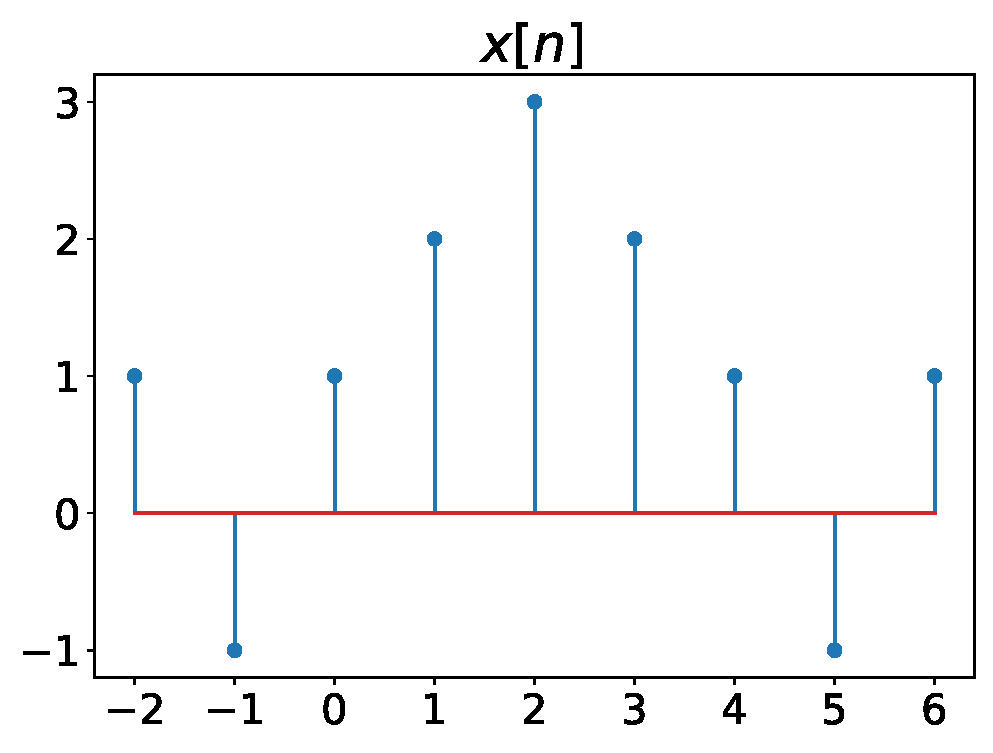
\includegraphics[width=80mm]{PS10_Q3.eps}
\end{figure}

در این صورت، موارد زیر را به کمک خواص تبدیل فوریه بیابید.

الف)
$
\int_{-\pi}^{\pi} X^2(e^{j\omega})d\omega
$

ب)
$
\int_{-\pi}^{\pi} \omega\left|{dX(e^{j\omega})\over d\omega}\right|^2d\omega
$

\newpage

\Q
برای سیگنال پیوسته‌ی
$
x(t)
$
با تبدیل فوریه‌ی زیر،

\begin{center}
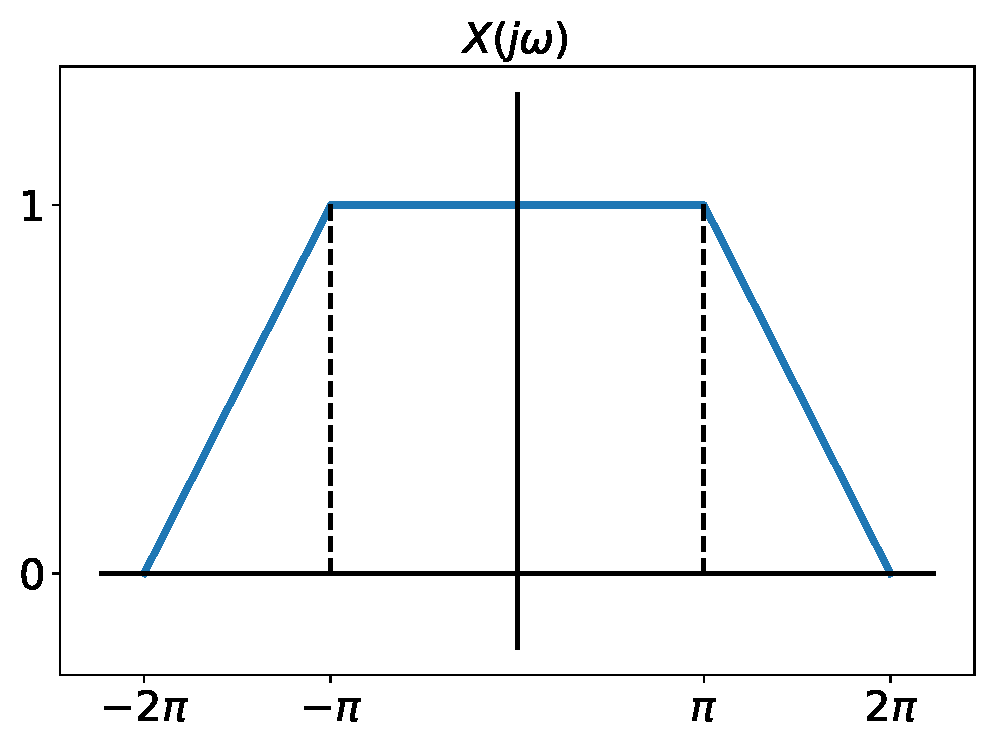
\includegraphics[width=70mm]{final1_samp.eps}
\end{center}

(محور افقی، نشان دهنده‌ی فرکانس زاویه ای $\omega$ است.)

الف) مقدار نرخ نایکوئیست را تعیین کنید و آن را با $F_s$ نشان دهید. سپس طیف سیگنال نمونه برداری شده با نرخ $2F_s$ را رسم کنید.

ب) فرض کنید سیگنال $x(t)$ را با نرخ 
$
\frac{3F_s}{4}
$
نمونه برداری کرده و آن را 
$
\hat x[n]
$
نامیده ایم. به عبارت دیگر
$$
\hat x[n]=x(\frac{t}{3F_s/4})
$$

اگر با بهره گیری از نمونه های 
$
\hat x[n]
$
، سیگنال پیوسته‌ی $y(t)$ را با نرخ نمونه برداری 
$
\frac{3F_s}{4}
$
بسازیم، آیا 
$
x(t)
$
با 
$
y(t)
$
برابر است؟

ج) (امتیازی) جزئیات ریاضی محاسبه‌ی $y(t)$ را انجام دهید.

% سیگنال پیوسته‌ی $y(t)$ را به گونه ای بیابید که دارای دو خاصیت زیر باشد
%$$
%|Y(j\omega)|=0\quad,\quad |\omega|>\pi \frac{F_s}{2}
%$$
%$$
%\hat y[n]=y(\frac{t}{F_s/2})=\hat x[n]
%$$

\newpage

%\Q
%یک سیستم گسسته، حقیقی و پایدار دارای خواص زیر است:
%\begin{itemize}
%\item
%تابع انتقال سیستم ($H(z)$) دارای 4 قطب است و صفر ندارد.
%\item
%پاسخ ضربه زوج است.
%\item
%یکی از قطب های تابع انتقال در 
%$
%z=\frac{1}{2}e^{j\frac{\pi}{4}}
%$
%قرار دارد.
%\end{itemize}
%
%پاسخ این سیستم به ورودی 
%$
%x[n]=2^nu[-n-1]
%$
% را در حوزه زمان بیابید.

\Q
ورودی متناوب 
$
x[n]=\sum_{k=-\infty}^\infty \delta[n-4k]-\sum_{k=-\infty}^\infty 2\delta[n-2k]
$
به سیستمی با پاسخ فرکانسی زیر داده شده است:
\begin{center}
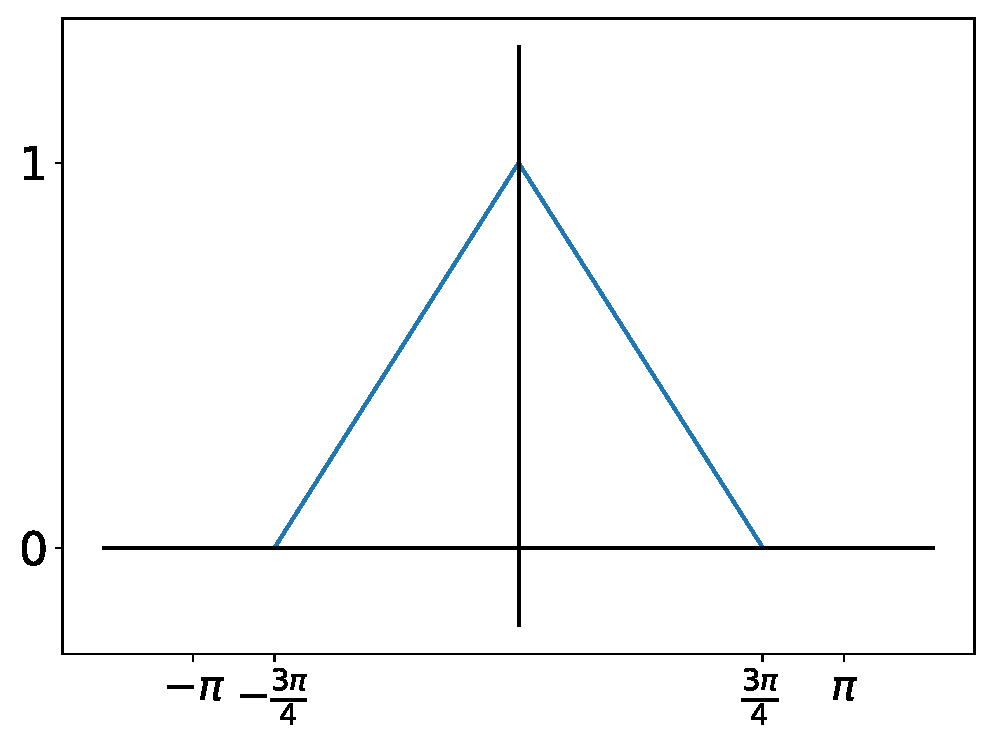
\includegraphics[width=80mm]{final_h2.eps}
\end{center}

پاسخ زمانی خروجی این سیستم را بیابید.

\newpage

\Q
تابع انتقال یک سیستم گسسته و LTI ، دارای نمودار صفر-قطب به صورت زیر است:

\begin{center}
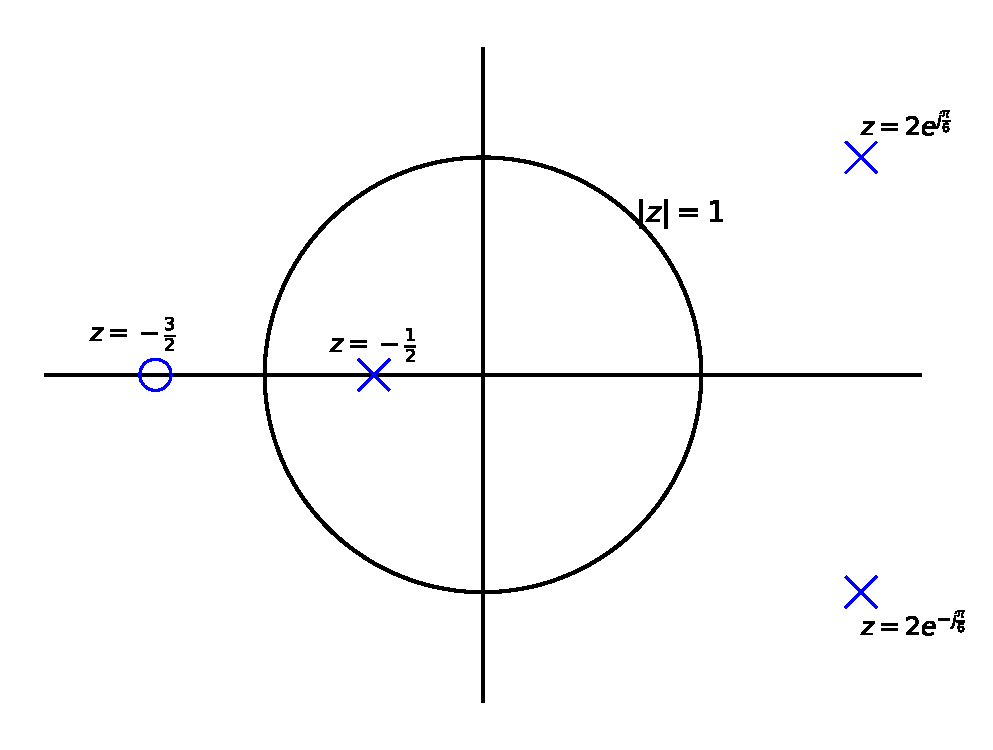
\includegraphics[width=100mm]{final_inv.eps}
\end{center}

الف) اگر سیستم علی باشد، رابطه‌ی زمانی پاسخ ضربه را بیابید.

ب) اگر سیستم پایدار و دارای وارون پایدار باشد، رابطه‌ی زمانی پاسخ ضربه‌ی سیستم معکوس را بیابید.
\end{document}